\section{Experimental Scope and Further Analysis}
\label{sec:limits}
\paragraph{Update design and attribution.}
The experimental comparison evaluates Block3 as an integrated block-level update: shared advantages, joint importance ratios and valid-length-weighted block reduction. Section~\ref{sec:method} characterizes the resulting cross-token credit, gradient scale and clipping geometry. Accordingly, the measured performance differences concern the complete update rather than advantage averaging alone. Component-specific attribution can be examined separately by holding ratios and normalization fixed when varying feedback sharing. The signal-estimation analysis describes averaging under explicit assumptions; task-level accuracy is measured by the benchmark evaluations.

\paragraph{Statistical unit and checkpoint reporting.}
Each reported arm uses one training seed. Paired-question intervals characterize evaluation uncertainty conditional on the trained checkpoints, rather than variability across training seeds. They are pointwise and use no multiple-comparison correction. Each AIME set contains 30 questions, so one additional solved question changes Pass@8 by 3.33 points. We retain the checkpoint trajectories alongside Step200, a common scheduled endpoint adopted retrospectively for reporting rather than a preregistered selection rule. Window and weighting variants arose through exploratory experiments; independent runs would evaluate the reproducibility of their observed differences.

\paragraph{Protocols and task coverage.}
Historical results are organized by their original prompt, seed-handling, teacher and implementation settings. Each stratum supplies a method comparison under its own protocol. The two fully retained comparisons share a DAPO-derived training pool; the overlap audit checks the retained data rather than semantic equivalence or upstream model exposure. The 4B completion study compares the two trained methods without a matched original-student evaluation, while the official Instruct pair additionally includes that control. Independent datasets, training seeds and teacher--student pairs provide natural axes for extending this evaluation.

\paragraph{Complementary diagnostics.}
Prompt probes examine behavior before optimization, while retained training trajectories characterize subsequent evolution. Entropy maps describe the prefixes visited by the current policy; missing boxed markers measure one specific formatting property. Gradient norms and length-stop rates track numerical and generation behavior, and sign disagreement measures how feedback is redistributed. Benchmark accuracy provides a separate task-level assessment. Interpreting these measurements jointly distinguishes input compatibility, optimization dynamics and mathematical correctness without treating one as a proxy for all three.

\paragraph{Baseline and computational scope.}
Sampled-token OPD is the matched experimental baseline; other OPD recipes are discussed as related work. Block3 changes how the available teacher feedback drives the update and still scores every valid response position. The present evaluation therefore concerns the behavior and accuracy of this update, not a reduction in teacher-scoring work. Per-task, per-checkpoint reporting captures the observed variation. Further comparisons can examine component choices and accuracy--cost trade-offs under a common budget.


\section{Additional Derivations}
\label{app:proofs}
\paragraph{The production reduction.}
Let $m_t\in\{0,1\}$ be the final actor mask, $n_b=\sum_{t\in b}m_t$, $N=\sum_t m_t$, and $\eta=10^{-8}$. Empty blocks have $\bar a_b=0$.
The code minimizes the negative clipped surrogate with a fractional block mask:
\begin{equation}
 L_{\mathrm{blk}}=-\frac{\sum_b(n_b/k)\mathcal C(R_b,\bar a_b)}{N/k+\eta}
 =-\frac{\sum_b n_b\mathcal C(R_b,\bar a_b)}{N+k\eta}.
\end{equation}
The token denominator is $N+\eta$. Invalid positions are zeroed before block aggregation; holes are not removed and do not move neighboring tokens into different blocks. Both empty blocks and padding have zero weight. With actor micro-batch size one, the update averages independently normalized response losses. It is not the batch-global token mean when response lengths differ. Thus the configuration label \texttt{token-mean} alone does not establish the global weighting used in DAPO \citep{dapo}.

\paragraph{Clipping convention.}
For lower and upper ratios $d=0.8$, $u=1.2$, define $s(r,a)=\min\{ra,\clip(r,d,u)a\}$. The inherited objective is
\begin{equation}
 \mathcal C(r,a)=\begin{cases}\max\{s(r,a),3a\},&a<0,\\s(r,a),&a\ge0.\end{cases}
\end{equation}
This is ordinary PPO clipping with an additional negative-advantage dual-clip rule. The block ratio is formed before applying this operation. Gradient-norm clipping at one is a separate optimizer operation. Neither operation is a guarantee that all future policy ratios or teacher KL values remain inside a prescribed region.

\paragraph{First-order derivatives and synthetic checks.}
On the active branch, for valid $t\in b$, the derivatives with respect to current sampled log probabilities are
\begin{equation}
 \frac{\partial L_{\mathrm{blk}}}{\partial\log p_\theta(y_t\mid h_t)}
 =-\frac{n_b\bar a_bR_b}{N+k\eta},\qquad
 \frac{\partial L_{\mathrm{tok}}}{\partial\log p_\theta(y_t\mid h_t)}
 =-\frac{a_tr_t}{N+\eta}.
\end{equation}
At ratio one, their policy loss values agree in the $\eta=0$ idealization for arbitrary advantages, yet their derivatives need not. For five tokens with $a_t=1$, the token derivatives are all $-1/5$, whereas Block3 gives $(-3/5,-3/5,-3/5,-2/5,-2/5)$. For $(a_1,a_2,a_3)=(1,-1,1)$, the token derivatives are $(-1/3,1/3,-1/3)$ and the block derivatives are $(-1/3,-1/3,-1/3)$. These are synthetic derivative examples, not estimates of real parameter-update magnitudes.

\paragraph{A restricted credit-horizon interpretation.}
Assume a fixed horizon $T$, a deterministic contiguous partition, no masks or truncation, locally parameter-independent student support on which the fixed teacher $q$ is positive, and sampling from the full current student distribution $p_\theta$. Suppose log probabilities are differentiable and differentiation and expectation can be interchanged. Define $c_t=\log p_\theta(y_t\mid h_t)-\log q(y_t\mid h_t)$ and $g_t=\nabla\log p_\theta(y_t\mid h_t)$. Then
\begin{align}
 \nabla\KL(P_\theta\Vert Q)
 &=\E\left[\left(\sum_t c_t\right)\left(\sum_t g_t\right)\right] \\
 &=\E\left[\sum_t g_t\sum_{u=t}^{T}c_u\right].
 \label{eq:fullcredit}
\end{align}
The derivative of the log-density term has expectation zero. Past terms vanish because $c_u$ for $u<t$ is measurable at $h_t$ and $\E[g_t\mid h_t]=0$. Define $H_{\mathrm{blk}}=\sum_b(\sum_{u\in b}c_u)(\sum_{t\in b}g_t)$ and $H_{\mathrm{seq}}=(\sum_u c_u)(\sum_t g_t)$. Applying the same argument to an unclipped block estimator at the old policy gives
\begin{equation}
 \E H_{\mathrm{blk}}=\E\left[\sum_t g_t\sum_{u=t}^{e(t)}c_u\right],\qquad
 \E(H_{\mathrm{seq}}-H_{\mathrm{blk}})=\E\left[\sum_t g_t\sum_{u>e(t)}c_u\right],
 \label{eq:horizon}
\end{equation}
where $e(t)$ is the end of token $t$'s block. Relative to purely local token feedback, block aggregation can restore within-block future credit; it omits credit across a block boundary. Thus cross terms should not all be called harmful leakage. Their omitted vector can cancel, so increasing block size need not monotonically reduce bias. MiniLLM already accounts for future rewards; this interpretation is not a claim to first introduce temporal credit assignment in distillation \citep{minillm}.

These identities do not establish that the production loss is an exact sequence-KL optimizer. Top-$p$ sampling changes the sampling distribution relative to the scored student; a product over masked positions is not generally a block marginal likelihood ratio; clipping and frozen old-policy targets alter the objective away from the old policy; and a random response length in the normalization introduces a dependence on future actions. The identities are therefore explanatory idealizations with explicit assumptions, not guarantees for the experiment.

\paragraph{Averaging error decomposition.}
With $a=\mu+\varepsilon$ and $\E\varepsilon=0$, expand $Wa-\mu=(W-I)\mu+W\varepsilon$.
The expected cross term vanishes, and $\E\varepsilon^\top W^\top W\varepsilon=\operatorname{tr}(W\Sigma W^\top)$, proving Equation~\ref{eq:mse}.
For independent, equal-variance noise and a constant signal within a $k$-token block, each averaged noise variance is $k\sigma^2/k^2=\sigma^2/k$.
For a deterministic signal $(2,-1,2)$ with zero noise, the unaveraged error is zero; replacing every component by its mean one creates squared error six. This is a counterexample to universal signal-estimation benefit, not a claim that the teacher's per-token ratio is always the correct task-level signal.

\paragraph{What sliding phases can average out.}
Let $X$ contain shared parameters, the collected batch, masks, frozen targets and all other forward randomness. Let $L_r(X)$ be the fully clipped and reduced loss for offset $r\in\{0,1,2\}$, and $G_r(X)=\nabla_\theta L_r(X)$. For a conditionally uniform random offset $U$, the implemented phase average satisfies
\begin{equation}
 G_{\mathrm{slide}}(X)=\frac13\sum_{r=0}^2G_r(X)
 =\E[G_U(X)\mid X].
\end{equation}
With finite second moments and the same distribution of $X$, the law of total covariance gives
\begin{equation}
 \Cov(G_U)-\Cov(G_{\mathrm{slide}})
 =\E_X[\Cov(G_U\mid X)]\succeq0.
 \label{eq:phasecov}
\end{equation}
This removes variance from offset randomization conditional on a common state; it does not compare Sliding3 with a fixed Block3 partition. PPO clipping may be active because it occurs inside each $L_r$. Gradient-norm clipping and Adam are nonlinear later operations and are outside this identity. Distinct training histories induce distinct distributions of $X$, so the identity is not a performance guarantee for the retained runs or an assertion about an exactly realized average under one fixed RNG seed. Averaging losses is also not the same as averaging advantages before a single clipping operation.

For $N>0$ and matching phase-zero partitions, $L_{\mathrm{hist}}=N L_0/(N+k\eta)$, including partial-tail weights. The gradients have the same factor because the collected mask is frozen. At $\eta=0$, the old reduction and phase-zero reduction are identical. Leading padding or holes can invalidate the matching-partition premise; floating-point operation order can introduce small numerical differences even when the ideal expressions agree.

\section{Configuration and Data Provenance}
\label{app:config}
\paragraph{Current model identities.}
The original student is \texttt{Qwen/Qwen3-4B-Base}, obtained from ModelScope at revision
\texttt{bbd6fc8d23e8788d987b7b970cbb7bd31c826e38}.
The public teacher's retained model card identifies \texttt{lllyx/Qwen3-4B-Base-GRPO}, released with Rethinking OPD \citep{rethinking}. That repository now redirects to \href{https://huggingface.co/Thinking-Space/Qwen3-4B-Base-GRPO}{\texttt{Thinking-Space/Qwen3-4B-Base-GRPO}}. It is a researcher's GRPO-adapted checkpoint, not an official Qwen instruction model and not a privately trained checkpoint from this project.
Download-cache metadata records revision \texttt{1f3b2966edfb75f2f98a00617588c1f748088422}; the two weight-file ETags match the retained asset hashes. The uploader's model card describes GRPO adaptation on DAPO-Math-17k-Processed. This upstream teacher training is distinct from our student's 200-update OPD runs.

\begin{table}[h]
\caption{Shared configuration for the current 4B completion comparison. Differences between training rollout inference and full evaluation are intentional and identical across arms.}
\centering\small
\begin{tabular}{@{}p{2.5in}p{2.65in}@{}}
\toprule
Setting & Value \\
\midrule
Training seed / data seed & 21 / 21 \\
Updates / prompts per update / samples & 200 / 4 / 8 \\
PPO mini-batch / epochs & 32 responses / 1 \\
Actor / rollout-logprob / teacher micro-batch & 1 / 4 / 1 per GPU \\
Optimizer / learning rate & AdamW / $2\times10^{-6}$ \\
Adam betas / epsilon / weight decay & $(0.9,0.999)$ / $10^{-8}$ / 0.01 \\
Schedule / warmup & Constant / zero warmup ratio \\
Gradient-norm clipping & 1.0 \\
PPO lower / upper clip / dual clip & 0.2 / 0.2 / 3.0 \\
Explicit entropy / extra KL loss & 0 / disabled \\
Outcome reward / OPD future-return weight & 0 / 0 \\
Teacher target log-ratio clipping & Disabled \\
Special-token OPD mask & Disabled; retain upstream response mask \\
Prompt cap / response cap & 2,048 / 16,384 \\
Temperature / top-$p$ / top-$k$ & 1.0 / 0.9 / unrestricted \\
Training rollout / eval memory fraction & 0.6 / 0.9 \\
Training max batched rollout tokens & 18,432 \\
Hardware / tensor parallelism & 4 A100-80GB / 1 \\
Training parameter / optimizer offload & Enabled / enabled \\
Gradient checkpointing & Enabled \\
Save steps / checkpoint deletion & 50, 100, 150, 200 / none \\
Diagnostic interval / top-$k$ / position bin & Every update / 16 / 128 tokens \\
Block sign threshold & $10^{-4}$ \\
\bottomrule
\end{tabular}
\end{table}

\paragraph{Exact completion prompt and stopping.}
Training and evaluation in the 4B Base comparison use the same completion function, without ChatML:
\begin{quote}\small
\texttt{[question]}\\
\texttt{Please solve the problem step by step and put the final answer in}\ \verb|\boxed{}.|\\
\texttt{Solution:}
\end{quote}
Blank lines separate the components, with a final newline after \texttt{Solution:}. Thinking is explicitly disabled, while ordinary step-by-step text is allowed. EOS is 151643 with no additional stop-token IDs. Actual input token IDs are checked after checkpoint merging. Evaluation runs on four independent tensor-parallel-size-one workers, using memory fraction 0.9 rather than the training rollout fraction 0.6. CPU checkpoint merging does not modify the original training weights. Raw responses, input tokens, request seeds and engine stopping reasons are retained.

\paragraph{Effective batching and seeds.}
Data batching follows the frozen seed-21 loader. Pair validation compares the actual source and prompt identities after collection; relying on equal seed labels alone would be insufficient if the arms consumed RNG differently. The current request-seed rule uses a stable SHA-256 derivation including step and sample identity and does not consume the training RNG merely to log a response. Eight requests for one prompt have separate seed identities. Historical fixed-request-seed runs are explicitly separated in Appendix~\ref{app:history}. A separate window-seed value is retained in the run card but has no effect on a fixed-block treatment.

\paragraph{Training pool.}
A direct read of the retained parquet verifies exact question--answer sequence repetition: a 17,917-row period occurs 100 times. There are 17,237 unique raw question strings and 17,249 unique raw question--answer pairs, without additional Unicode or mathematical normalization. These are exact-string counts, not semantic deduplication. The original expansion command and upstream dataset revision were not recovered. The retained file's SHA-256 starts with \texttt{cf359f257a320aecb}; the internal manifest preserves the complete digest. No claim of comprehensive train--test semantic decontamination follows from hashing. Both methods nevertheless use exactly the same retained pool, rather than separately downloading whichever dataset version currently bears the same name.

The retained converter names \texttt{BytedTsinghua-SIA/DAPO-Math-17k}, file \texttt{data/dapo-math-17k.parquet}, as its public default input. However, the historical manifest records a copied, already converted parquet, not its original Hub revision or the command that created the 100-fold expansion. The current converter's default deduplication would change this pool. Its current defaults must not be presented as the exact historical preprocessing recipe.

\paragraph{Retrospective string-overlap audit.}
Comparing the original question fields, two of MATH500's 500 questions occur exactly in the retained training pool. Collapsing Unicode whitespace to single spaces, stripping boundaries and applying Unicode casefold yields four matches in total, including those two. This normalization does not rewrite mathematics or LaTeX. The exact held-out indices are 80 and 276; normalized-only additions are 285 and 412 (zero-based indices in the retained MATH500 artifact). The corresponding counts for AIME24, AIME25 and AMC23 are zero under both rules. We use the previously verified 17,917-row period to cover the pool's string set and check evaluation-file hashes and question-field identities. This is a retrospective data audit, not a filtering intervention: all reported full-benchmark scores retain the original questions. Pool membership alone does not demonstrate actual exposure during these 200 updates; string-level zero overlap does not establish semantic decontamination or audit the teacher's training/pretraining corpus.

A separate audit streams the actual retained input metadata from all 400 compressed training archives, verifies their recorded hashes, and compares both methods' complete 6,400-entry input streams. Each arm contains 800 prompt occurrences, 783 exact unique question strings and 782 whitespace/casefold-normalized strings. There are zero exact evaluation-question exposures and one normalized-only occurrence: MATH500 index 412 at Step71, eight trajectory records per arm. The other three pool-overlap candidates are absent. Both arms encounter the same input at the same step; Step50 precedes that exposure. This observation does not audit semantic equivalents or upstream model training. The separate 496-question sensitivity analysis excludes all four pool-matched items, independently of which happened to be drawn, while retaining full MATH500 as the primary report.

\paragraph{Evaluation artifacts and grading.}
MATH500 uses the \texttt{HuggingFaceH4/MATH-500} test artifact, related to the MATH and PRM800K evaluation lineage \citep{math,prm800k}. AIME24 was converted from \texttt{BytedTsinghua-SIA/AIME-2024}. AIME25 and AMC23 were converted from the corresponding retained test parquet files in the public OPD repository. Their local counts are respectively 30 and 83; in particular, the AMC23 count must not be silently equated with another paper's 40-question subset. The converted JSONL hash prefixes are \texttt{cc164b47b60771ee} (MATH500), \texttt{6aee5ed24b811ebc} (AIME24), \texttt{daedf1e406b9d73c} (AIME25), and \texttt{a07c52c0098a536a} (AMC23).

The same historical external grader, SHA-256 prefix \texttt{04f7a0328be18409}, scores both arms. Eight independently seeded generations are retained for each question. Every finalized checkpoint checks the expected question identities, response counts, raw output archives, and agreement between summary and graded records. This validates the evaluation contract, not the logical infallibility of the symbolic grader. Grader errors or missing parseable answers must not be reinterpreted as known mathematical correctness. Missing boxed-answer markers and engine length stops remain separate measurements.

The public repository for the two retained parquet sources is \url{https://github.com/thunlp/OPD}, checkout \texttt{1fd6cca846126af90d82ef122e8af261f59d2d37}, at \path{datasets/test_data/AIME25/test.parquet} and \path{datasets/test_data/AMC23/test.parquet}. The checked-out files match the historical source hashes. Their more remote upstream Hub namespaces were not recovered. This data-source repository is distinct from the Revisiting OPD training codebase.

\paragraph{Resource accounting and retention.}
The two current 200-step training runs took approximately 9.4 and 9.7 hours on four A100 GPUs, excluding evaluation and bounded acceptance probes. This is roughly 76 GPU-hours of training for this pair, not an estimate of the entire project's compute. Total historical compute cannot be reconstructed from the retained summaries with comparable precision. All four full states per arm, including optimizer, scheduler and RNG state, remain retained. Each current arm has 200 diagnostic records and 6,400 raw training trajectories. Some early experiments did not save raw training trajectories; sampling an old checkpoint now would not recover those original rollouts.

\paragraph{Software and precision.}
The retained runtime uses Python 3.12.13, PyTorch 2.8.0, vLLM 0.11.0, Transformers 4.57.6, Ray 2.55.1, NumPy 1.26.4, Datasets 4.8.5 and OmegaConf 2.3.0. These versions were read from the evaluation environment; they are not inferred from a current package installation guide. The unchanged FSDP actor defaults load the training model in float32 and use bfloat16 forward parameters with float32 reduction and buffers; the reference model and rollout inference use bfloat16. Both arms use the same frozen runtime and model/tokenizer bytes. A generic tokenizer-regex warning was retained, not patched in only one arm during evaluation; the acceptance gate checks the actual prompt token IDs for the paired protocol. This check establishes matched behavior, not that arbitrary prompts are immune to tokenizer defects.


\section{Diagnostic Definitions}
\label{app:diagnostics}
\paragraph{Entropy and occupied prefixes.}
At a valid student-generated prefix $h_t$, let $p_t(v)$ and $q_t(v)$ be the student and teacher softmax distributions over the shared vocabulary. We record full-vocabulary Shannon entropies in nats,
\begin{equation}
 H_{\mathrm S,t}=-\sum_v p_t(v)\log p_t(v),\qquad
 H_{\mathrm T,t}=-\sum_v q_t(v)\log q_t(v).
\end{equation}
The configured temperature is one. These are not entropies of a renormalized top-16 support, nor negative log probabilities of the one sampled token. The signed gap is $H_{\mathrm T,t}-H_{\mathrm S,t}$; the absolute gap is the absolute value at each position, averaged afterward. Therefore the mean absolute gap is not generally the absolute value of the mean signed gap. Student and teacher are evaluated on the same student prefix. Their training-time snapshots are taken before the update for that batch; appended optimizer and post-update ratio diagnostics describe a different phase of the same update.

\paragraph{Top-token alignment.}
Let $S_t$ and $Q_t$ be the respective top-16 token-ID sets and $O_t=S_t\cap Q_t$. We compute
\begin{equation}
 \mathrm{Overlap}_t=|O_t|/16,\quad
 M_{\mathrm S,t}=\sum_{v\in O_t}p_t(v),\quad
 M_{\mathrm T,t}=\sum_{v\in O_t}q_t(v).
\end{equation}
Probability masses use the original full-vocabulary probabilities. They are not percentages of the top-16 mass. When $O_t\ne\varnothing$, the implemented overlap-token advantage first renormalizes within the intersection:
\begin{equation}
 \bar p_t(v)=p_t(v)/M_{\mathrm S,t},\quad
 \bar q_t(v)=q_t(v)/M_{\mathrm T,t},\quad
 U_t=\frac{1}{|O_t|}\sum_{v\in O_t}\bar p_t(v)
       \log\frac{\bar q_t(v)}{\bar p_t(v)}.
\end{equation}
Thus $U_t=-\KL(\bar p_t\Vert\bar q_t)/|O_t|\le0$ in exact arithmetic; it is not the average raw sampled-token advantage. Empty intersections are excluded from its mean, while their overlap ratio and masses are zero. We state the implemented definitions rather than assuming every diagnostic with the same name in another paper uses identical normalization.

\paragraph{Local sign disagreement and redistribution.}
Let $b_t$ be the block mean copied to valid token $t$, $m_t$ the recorded response mask, and $\epsilon=10^{-4}$. Define
\begin{align}
 e_t&=m_t\mathbf1[|a_t|>\epsilon]\mathbf1[|b_t|>\epsilon],\\
 f_t&=e_t\mathbf1[\operatorname{sign}(a_t)\ne\operatorname{sign}(b_t)].
\end{align}
The recorded sign-flip rate and its magnitude-weighted variant are
\begin{equation}
 F=\frac{\sum_t f_t}{\max(1,\sum_t e_t)},\qquad
 F_w=\frac{\sum_t |a_t|f_t}{\max(\epsilon,\sum_t |a_t|e_t)}.
\end{equation}
Tokens with near-zero local or shared feedback are not classified as direction reversals. A batch with no eligible entries yields zero together with zero coverage, not evidence that all directions agree. The redistribution statistics are
\begin{equation}
 D=\frac{\sum_t m_t|b_t-a_t|}{\max(1,\sum_t m_t)},\qquad
 D_{\mathrm{rel}}=\frac{\sum_t m_t|b_t-a_t|}{\max(\epsilon,\sum_t m_t|a_t|)}.
\end{equation}
The source calls these quantities \texttt{leakage\_magnitude} and \texttt{normalized\_leakage}. We use ``redistribution'' because neither difference from token feedback nor a sign reversal proves harmful task-level credit. These statistics also do not include the joint-ratio derivative or its effective scale. For a size-one Token treatment, $b_t=a_t$ and both families vanish by construction; this is not independent evidence of superior training behavior.

\paragraph{Position aggregation and missingness.}
For every update, the retained snapshot stores sums, squared sums and valid counts at generated response positions, using the diagnostic response mask. In the current completion run, the historical EOS mask includes the first EOS (151643), excludes subsequent positions and the prompt, and includes every position of a cap-length response without EOS. The figures combine consecutive positions into bins of 128 tokens using ratios of sums to counts, not an unweighted average of precomputed means. Alignment is sampled at stride one. Sign-flip heatmaps use eligible counts rather than all response-token counts. A displayed bin must have at least one original position with eight valid observations; the threshold is applied to the maximum per-position count inside the bin, not to its summed token count. A gray masked cell is not zero entropy or zero disagreement. A bin's denominator counts token-position observations and need not equal the number of distinct trajectories. The changing density of long responses is shown separately from the measured values. Comparing two bins or training steps conditions on different on-policy prefixes and therefore cannot on its own establish which process caused collapse.

\paragraph{Optimizer, lengths and format.}
The recorded gradient norm is the worker's norm before configured norm clipping, reduced by the training logger; it is not a measurement that every token-specific or layer-specific derivative remains bounded. Policy-gradient loss is the actual clipped objective, which need not be directly comparable in scale between Token and Block3. Training response-cap incidence counts trajectories that reach the configured cap. For evaluation we additionally retain the engine's length-stop reason; a cap statistic based on a mask and an engine stopping reason should not be assumed identical without checking.

Our format indicator is the evaluation wrapper's literal test that the response does not contain the string \verb|\boxed|. It does not validate brace balance, extractability or whether the box contains the final answer. It is narrower than ``the answer has any formatting defect,'' and it is separate from incorrect arithmetic, symbolic grading failure, malformed thinking tags and length termination. A response can contain the marker and still be incorrect; a length-stopped response may already contain it. All rates use the relevant benchmark's retained response count. We make no cross-benchmark aggregate formatting claim.


\section{Historical Evidence and Protocol Boundaries}
\label{app:history}
\begin{table}[htbp]
\centering\small
\caption{Complete historical Step200 Avg@8 comparison (\%). Original prompts and protocols are retained; compare methods only within each student stratum. These are not extra training seeds of the two fully retained comparisons.}
\label{tab:historyendpointsfull}
\begin{tabular}{@{}llrrrr@{}}
\toprule
Student & Method & MATH500 & AIME24 & AIME25 & AMC23 \\
\midrule
Qwen 1.7B & Token & 45.85 & 5.42 & 2.50 & 21.84 \\
Qwen 1.7B & Block3 & 54.75 & 8.75 & 5.42 & 27.26 \\
\addlinespace
DeepSeek 1.5B & Token & 84.70 & 39.58 & 29.17 & 73.34 \\
DeepSeek 1.5B & Block3 & 84.75 & 43.75 & 30.83 & 73.80 \\
\addlinespace
Qwen 0.6B & Token & 42.88 & 2.50 & 0.83 & 18.98 \\
Qwen 0.6B & Block3 & 0.57 & 0.00 & 0.00 & 0.45 \\
\addlinespace
Llama 1B & Token & 15.55 & 0.42 & 0.00 & 6.02 \\
Llama 1B & Block3 & 6.30 & 0.00 & 0.00 & 1.51 \\
\addlinespace
\bottomrule\end{tabular}

\end{table}
\paragraph{Inventory and evidence strength.}
The historical inventory contains 17 experimental series and 171 evaluation records, including alternative grader views and explicit missing results. It is not a count of 171 independent training runs. Below, percentages are reported separately for each benchmark. A dash means that no completed result was recovered, not zero accuracy. In the n=8 tables, cells contain Avg@8 / Pass@8. The early n=1 and 100-question pilot tables retain their original metric definitions. Regrading the same generations does not add samples, and re-evaluating an old checkpoint does not add a training seed.

The strongest retained evidence consists of original evaluation summaries with their acceptance records. Other tables come from finalized paired artifacts or curated summaries. The earliest block-sum and block-advantage results are available only as rounded values in historical reports; we retain that limitation rather than reconstructing exact counts from rounded percentages. Source paths and identifying infrastructure information remain outside the anonymous manuscript. A complete internal provenance map records which fields support each value.

\paragraph{H01--H05: clean-room exploration.}
The earliest student and teacher were the official post-trained \texttt{Qwen3-0.6B} and \texttt{Qwen3-4B}, not their Base variants and not the later GRPO teacher. The 3,400-prompt training pool combined 2,000 GSM8K training examples with 200 training examples from each of MATH's seven subjects. Small weighting pilots, outcome weighting, reference anchoring, naive block sums, and sum/mean/mixed variants were explored. Full evaluation meant GSM8K's 1,319 test examples and 500 MATH examples, n=1, with a 256-token output cap, temperature 0.7 and top-$p=0.95$. The 100-example pilots are not full evaluations and their sample-count parameter is not recoverable from those summaries.

These runs use a different loss family from the main study. The clean-room implementation applies detached weights and advantages to summed current log probabilities without a PPO ratio, clamps its raw signal, and discards incomplete blocks. Its mixed mode interpolates token-local and block-mean signals; this is not the later block-sum/block-mean interpolation option. Exact settings for some named router or anchor variants are incomplete. Consequently, the old pilot tables document the research trajectory and negative outcomes, not replications of the current loss or implementations of similarly named external papers. Outcome weighting did not prevent endpoint degradation: the two reweighted 200-step arms attain primary-grader MATH500 accuracies of 16.60\% and 16.40\%, below the recorded 20.20\% initial reference; the standard arm attains 14.80\%. Missing intermediate reweighted evaluations prevent locating the onset of that degradation. The standard arm's Step50 entry in an older composite chart came from an earlier pilot and is not connected here as if it were the same training run.

\paragraph{H06--H09: size sweep, collapse and Qwen 1.7B.}
The DAPO-era Qwen3-1.7B-Base student uses the retained 4B GRPO teacher. The original block-size sweep mixed hardware contexts and did not explicitly fix evaluation seeds in every older invocation. Token, Block3 and Block5 used A800 hardware; Block10 used A100 hardware. The retained Step200 Avg@8 / Pass@8 table for $k\in\{1,3,5,10\}$ appears in Appendix~\ref{history:qwen17_sweep}. Block3 exceeds Block5 on every Avg@8 metric and on three Pass@8 metrics, tying AMC23 coverage. Its comparison to Token is mixed, so the sweep motivates retaining a short block rather than claiming universal superiority. The Block5 scores survive as a curated summary rather than recovered original evaluation files. The first Block5 attempt stopped at Step42 with a vLLM OOM; the successful restart lowered the rollout-memory fraction to 0.6. These resource changes must not be hidden when interpreting the sweep.

An earlier clean-room pilot compared $k\in\{1,2,3\}$ at 50 updates (Appendix~\ref{history:early_blocksum50}). Its recorded GSM8K/MATH500 accuracies were 45.94/20.00 for Token, 45.41/19.40 for Block2 and 46.85/20.20 for Block3. It used official 0.6B/4B post-trained models and a non-PPO loss, so this is preliminary motivation, not a $k=2$ result for the later 1.7B PPO implementation. No completed $k=2$ arm exists in the retained 200-step sweep.

The later same-host Token/Block3 comparison provides the cleaner historical method comparison. At Step200, its MATH500 Avg@8 changes from 45.85\% to 54.75\%, AIME24 from 5.42\% to 8.75\%, AIME25 from 2.50\% to 5.42\%, and AMC23 from 21.84\% to 27.26\%. Intermediate checkpoints are not uniformly favorable. Six later checkpoint evaluations regenerate outputs for the same Token/Block3 weights; these are evaluation sensitivity records, not six new training runs.

Both 1.7B arms use ChatML and request \texttt{<think>...</think>} during training without explicitly disabling thinking in the template kwargs. Evaluation uses ChatML with thinking disabled and no instruction requiring those tags, retaining the already-closed empty thinking-control prefix. The old collector resets the per-request training seed to 21, so nominal eight-response groups may contain duplicates. The original full training-token trajectories were not retained, preventing retrospective measurement of their exact duplicate rate. These shared historical choices do not become the current completion protocol merely because the dataset and global seed match.

The Block10 diagnostic repetitions both use training seed 21, one on A800 hardware and one on A100 hardware. Both record zero scores on all four benchmarks at Step200 while available optimizer diagnostics remain finite. Their grader is the legacy built-in VERL path, not the pinned external path used for the current comparison. In particular, built-in AMC23 zero scores have a known compatibility caveat and cannot independently establish absence of AMC capability; we retain them as historical outputs, not validated capability measurements. The severe generation degradation and failures on the other tasks remain relevant observations. These are two hardware-context repetitions, not a multiple-training-seed confidence estimate. Neither the scalar summaries nor these endpoints prove a unique cause such as gradient explosion, teacher unreliability, or reverse-KL mode collapse.

Table~\ref{tab:block10health} makes the limitation of a set-overlap diagnostic concrete: the two runs retain top-16 overlap ratios near 0.8 at Step200, while the shared tokens carry only about 0.17--0.24 of the full probability mass. High rank-set overlap need not imply concentrated agreement. The largest finite pre-clipping gradient norms occur at different steps (191 on A800 and 1 on A100), so these summaries do not support one reproducible temporal ordering of collapse.
\begin{table}[ht]
\centering\small
\caption{Retained Block10 diagnostic summaries. Entropies (nats), overlap ratio and intersection probability masses are measured at Step200; the last column is the maximum pre-clipping gradient norm over each run. Values come from the archived diagnostic report rather than a fresh training replication.}
\label{tab:block10health}
\begin{tabular}{@{}lrrrrrr@{}}
\toprule
Hardware & $H_S$ & $H_T$ & Overlap & $M_S$ & $M_T$ & Max. grad \\
\midrule
A800 & 7.146 & 6.745 & 0.837 & 0.226 & 0.237 & 867.495 \\
A100 & 7.576 & 6.962 & 0.793 & 0.166 & 0.186 & 865.207 \\
\bottomrule\end{tabular}

\end{table}

\paragraph{H10--H11: another distilled pair and alternative windows.}
The DeepSeek-R1-Distill-Qwen-1.5B/JustRL pair is a separate released-model comparison and still has a Qwen-derived backbone; it is not a new non-Qwen architecture. Its Step200 Avg@8 differences favor Block3 by 0.05, 4.17, 1.67 and 0.45 percentage points on MATH500, AIME24, AIME25 and AMC23, respectively. However, Step200 Pass@8 decreases on MATH500 and AIME24; Step50 AIME24/AMC23 and Step100 AIME25 also contain regressions. The archived protocol classifies this as a failed directional replication: its original criterion required positive equally weighted task-mean differences for both Avg@8 and Pass@8. We preserve that historical decision without using an aggregate score in the present tables. Positive Avg@8 endpoints should neither erase the failed criterion nor be described as uniformly negative. One training seed does not establish general transfer; all task/checkpoint views remain available.

Random3 and Sliding3 were trained and evaluated as their own pair at Steps 50, 100 and 200. Random3 chooses one of three partition offsets per update using a saved PCG64 RNG (seed 910021); Sliding3 averages the three complete offset-specific losses, after each phase's PPO clipping. Both retain partial edge windows. Their length-weighted phase-zero loss is algebraically equivalent to historical Block3 when valid responses start at position zero with right padding and the $10^{-8}$ denominator stabilizer is ignored. It would be misleading to call this a fundamentally different normalization. The implementation restarts coordinates at mask-separated valid regions and changes floating-point summation, so arbitrary masks need not give identical partitions. Each still performs one optimizer update per batch. A late advantage of Sliding3 over Random3 does not establish superiority over a newly matched fixed Block3 or Token control. Both alternatives can deteriorate during training. The archived grader recovery changes evaluation plumbing, not the frozen training run. Corrected external views support method comparisons; older built-in views remain explicitly separate, including the AMC23 grading caveat above.

\paragraph{H12--H15: small Base and instruction-tuned students.}
The old Qwen3-0.6B-Base attempt trained Token OPD but its Step50 evaluation was stopped during truncation diagnosis; no corresponding Block3 training is claimed. A later paired experiment explicitly disables thinking and retains ChatML, with both arms using the same repaired non-thinking protocol. This repair also changes the EOS stopping set and masks according to actual generated lengths; it is not a prompt-only intervention relative to the older run. It produces a strong negative transfer result for Block3: its Step200 MATH500 Avg@8 is 0.57\%, versus 42.88\% for Token. The 1.7B result is therefore not a universal argument for using blocks in smaller students.

The Llama pair is \texttt{Llama-3.2-1B-Instruct} and \texttt{Llama-3.2-3B-Instruct}, obtained as ModelScope mirrors of the same Meta release \citep{llama32}. It is not a 3.1 teacher paired with a 3.2 student, and neither checkpoint is a Base model. In the first native-prompt attempt, initial-model evaluation completed but Token training was deliberately stopped at Step146. A new pair then reproduced the historical 1.7B training/evaluation instruction difference while retaining Llama-native role boundaries. Token and Block3 complete 200 steps in this setting, with Block3 substantially worse on MATH500 and AMC23. The thinking flag is not a native Llama mode switch; an instruction asking for think tags is separate from the tokenizer's role format.

Both the 0.6B and Llama training series retain the old per-request fixed seed 21. Archived groups show that the eight nominal training responses to one prompt can be duplicates, so 6,400 retained trajectories do not imply 6,400 independent generations. The current completion comparison repairs this request-level seed rule. This training-sampling limitation is distinct from the eight independently seeded evaluation responses. It applies to interpreting effective exploration, not to retroactively changing any recorded benchmark score.

\paragraph{H16--H17: pre-update repetition and the completion restart.}
The 4B Base-model ChatML attempt was stopped after four updates. Repetition and length-cap hits were already present in its initial pre-update outputs, so those initial failures cannot be caused by its later Block3 gradients. Bounded prompt diagnostics examined native input token IDs, thinking instructions, EOS handling and request-seed reuse. The subsequent completion protocol simultaneously removes ChatML and uses independently derived per-request seeds. It is an engineering repair with matched new Token/Block3 arms, not a single-factor causal ablation of role tokens.

A first formal restart failed before its first update with a temporary-directory cleanup error on network storage. The retry moved compiler/temporary caches to executable shared memory while retaining the frozen training code and model/data contract. The failed attempt and its first trajectories remain retained. CPU/GPU acceptance probes that save and resume Steps1--2 are recorded as technical acceptance, not as extra benchmark experiments. The current pair's final results appear in Appendix~\ref{app:current}, replacing the pre-evaluation snapshot in this historical inventory.

\paragraph{Archive inclusion.}
The tables report completed evaluations with retained result artifacts; diagnostic probes and interrupted attempts are identified separately. Later checkpoint sampling is recorded as a new evaluation, not as recovery of the original training trajectories. The interpretation of the integrated update and directions for further comparisons are discussed in Appendix~\ref{sec:limits}.

Table~\ref{tab:historyendpointsfull} includes all four historical endpoint comparisons; Table~\ref{tab:historyendpoints} selects two positive Avg@8 examples for the main text. The following figures and tables retain the complete checkpoint trajectories.
\begin{figure}[p]
\centering
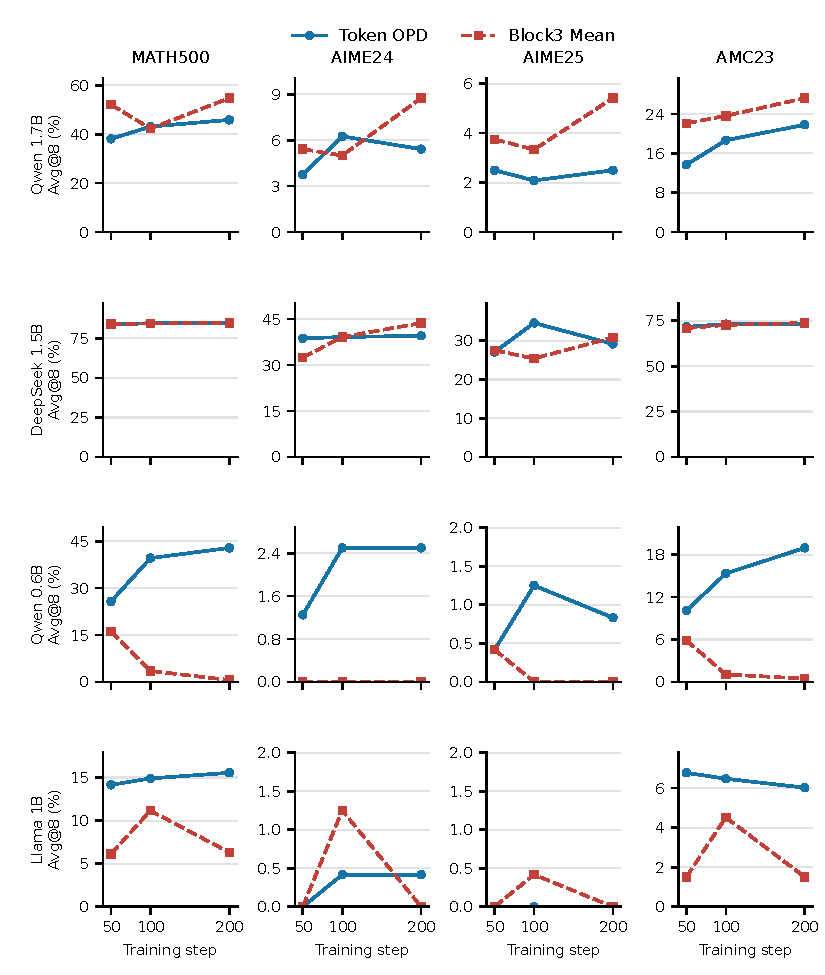
\includegraphics[width=\linewidth]{figures/history_20260921/history_avg_at_8.pdf}
\caption{Historical Avg@8 checkpoint trajectories, using the audited external view for Qwen 1.7B and the retained historical external view for the other strata. Each row keeps its own protocol; all use one training seed, not independent multi-seed replications. Panel scales differ. Lines only connect the three measured checkpoints and do not represent measurements between them.}
\label{fig:historyavg}
\end{figure}
\begin{figure}[p]
\centering
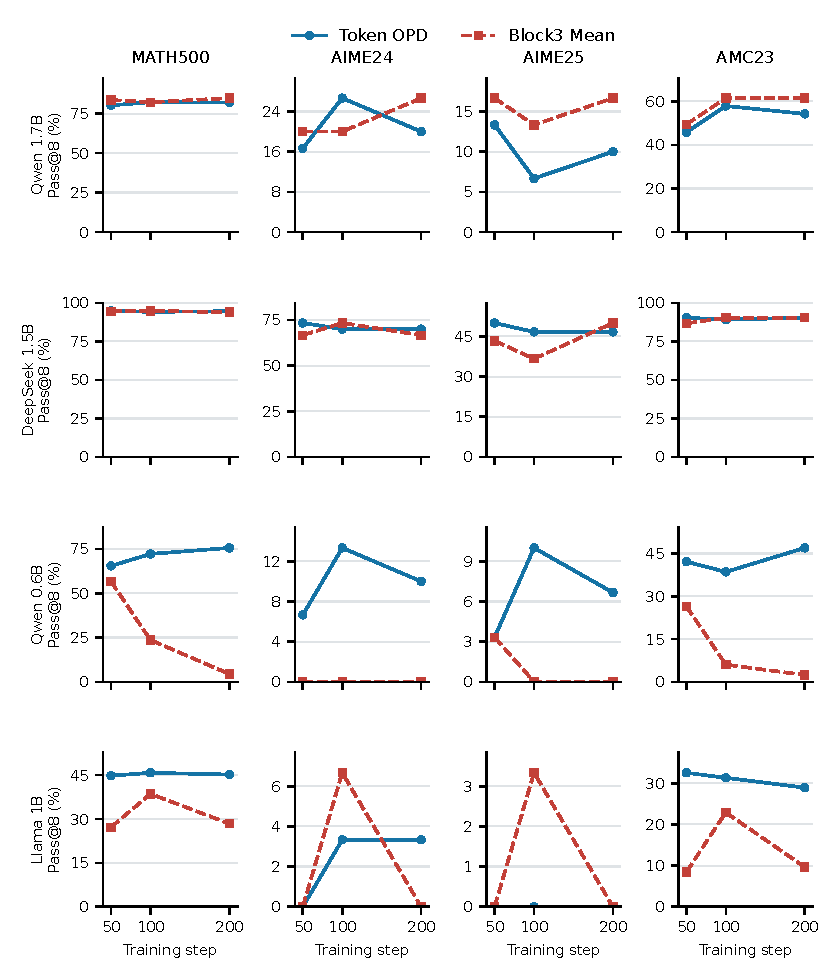
\includegraphics[width=\linewidth]{figures/history_20260921/history_pass_at_8.pdf}
\caption{Historical Pass@8 for the same checkpoints and protocol strata as Figure~\ref{fig:historyavg}. Each question contributes one if at least one of its eight evaluation responses is correct. This coverage statistic is distinct from averaging the eight correctness indicators. No interval over independent training seeds is implied.}
\label{fig:historypass}
\end{figure}
\clearpage
\input{generated/history_all_en}

\section{Bounded Prompt Diagnostics}
\label{app:probes}
These are inference probes on selected training questions, not additional held-out benchmark scores. The Qwen3-4B and Llama prompt studies use 16 fixed questions with two independently seeded responses per condition (seeds 21 and 22). Qwen 0.6/1.7 primary and first-16 ablation cells retain their separate sample counts; overlapping questions are not summed as independent observations. The tables contain integer counts: length stops, periodic tails, missing literal boxed markers and correctly graded responses. A dash indicates an unrecorded statistic. A periodic tail requires at least 256 retained tail tokens and an offset of at most 128 with at least 99\% token agreement within the last 2,048 tokens; it is a detector, not a general semantic repetition measure.

The historical training user message is:
\begin{quote}\small
\texttt{Math problem: [question]}\\
\texttt{Please carefully reason through the math problem step by step and derive the correct answer. You must conduct reasoning inside <think> and </think> and give the final answer within}\ \verb|\boxed{}.|\
\end{quote}
The native model template wraps that content with an assistant generation prefix. ``No think'' deletes only the phrase \texttt{conduct reasoning inside <think> and </think> and}; it is not the same as bypassing a chat template. Historical evaluation instead uses the question and \texttt{Please reason step by step, and put your final answer within} \verb|\boxed{}.|, with thinking explicitly disabled. Thus asking for reasoning tags and disabling a native thinking mode are distinct controls.

For Qwen3-4B, ``plain'' is the bare question followed by two newlines and \texttt{Solution:}; ``candidate'' is the final matched completion protocol in Section~\ref{sec:protocol}. For Llama, ``completion'' retains the non-think historical instruction and a single native BOS, removes chat role boundaries, and appends \texttt{Solution:}; it is not exactly the Qwen plain condition. The ``eval'' cell uses Llama's native non-thinking evaluation template. Removing chat raises Llama student length stops from 1/32 to 4/32 in this probe, while Qwen3-4B's historical-to-candidate change reduces them from 18/32 to 1/32. These observations motivate model-specific validation, not a universal rule to remove chat from instruction-tuned models.
\paragraph{Llama prompt}
{\small\setlength{\tabcolsep}{4pt}
\begin{longtable}{@{}llrrrrr@{}}
\toprule
Model & Condition & $n$ & Length & Periodic & No box & Correct \\
\midrule\endhead
student & historical & 32 & 1 & 1 & 10 & 0 \\
student & no\_\allowbreak{}think & 32 & 1 & 0 & 16 & 1 \\
student & completion & 32 & 4 & 1 & 3 & 1 \\
student & eval & 32 & 1 & 1 & 11 & 0 \\
teacher & historical & 32 & 2 & 1 & 6 & 3 \\
teacher & no\_\allowbreak{}think & 32 & 4 & 2 & 9 & 2 \\
teacher & completion & 32 & 4 & 2 & 2 & 1 \\
teacher & eval & 32 & 0 & 0 & 6 & 2 \\
\bottomrule\end{longtable}
}
\paragraph{Qwen3-4B prompt}
{\small\setlength{\tabcolsep}{4pt}
\begin{longtable}{@{}llrrrrr@{}}
\toprule
Model & Condition & $n$ & Length & Periodic & No box & Correct \\
\midrule\endhead
student & historical & 32 & 18 & 17 & 21 & 1 \\
student & plain & 32 & 0 & 0 & 9 & 2 \\
student & candidate & 32 & 1 & 1 & 0 & 4 \\
teacher & historical & 32 & 2 & 0 & 2 & 6 \\
teacher & plain & 32 & 0 & 0 & 0 & 5 \\
teacher & candidate & 32 & 3 & 2 & 2 & 8 \\
\bottomrule\end{longtable}
}
\paragraph{Qwen 0.6/1.7 primary32}
{\small\setlength{\tabcolsep}{4pt}
\begin{longtable}{@{}llrrrrr@{}}
\toprule
Model & Condition & $n$ & Length & Periodic & No box & Correct \\
\midrule\endhead
q06\_\allowbreak{}base & -- & 32 & 12 & 10 & -- & 0 \\
q06\_\allowbreak{}step50 & -- & 32 & 10 & 4 & -- & 1 \\
q17\_\allowbreak{}base & -- & 32 & 16 & 10 & -- & 1 \\
q17\_\allowbreak{}step50 & -- & 32 & 4 & 0 & -- & 4 \\
\bottomrule\end{longtable}
}
\paragraph{Qwen 0.6/1.7 prompt\_\allowbreak{}ablation\_\allowbreak{}first16}
{\small\setlength{\tabcolsep}{4pt}
\begin{longtable}{@{}llrrrrr@{}}
\toprule
Model & Condition & $n$ & Length & Periodic & No box & Correct \\
\midrule\endhead
q06\_\allowbreak{}base\_\allowbreak{}no\_\allowbreak{}think & -- & 16 & 5 & 4 & -- & 1 \\
q06\_\allowbreak{}base\_\allowbreak{}plain & -- & 16 & 1 & 1 & -- & 1 \\
q06\_\allowbreak{}base\_\allowbreak{}training & -- & 16 & 6 & 6 & -- & 0 \\
q17\_\allowbreak{}base\_\allowbreak{}no\_\allowbreak{}think & -- & 16 & 1 & 1 & -- & 1 \\
q17\_\allowbreak{}base\_\allowbreak{}plain & -- & 16 & 0 & 0 & -- & 0 \\
q17\_\allowbreak{}base\_\allowbreak{}training & -- & 16 & 6 & 4 & -- & 1 \\
\bottomrule\end{longtable}
}


\section{Complete 4B Base Checkpoint Results}
\label{app:current}
The current pair uses the matched completion protocol in Appendix~\ref{app:config}. Scores are percentages, not fractions. Differences subtract Token from Block3 at the same checkpoint and on the same benchmark. Missing-box-marker rates and engine length-stop rates use all eight responses per question; Avg@8 and Pass@8 have the definitions in Equation~\ref{eq:metrics}. Checkpoint comparisons describe a single training trajectory per method and should not be interpreted as independent repetitions.
\input{\qwenresults/qwen4_results_en}

Paired-question bootstrap intervals, where reported, resample the same question identities for both arms, separately within each benchmark. They condition on the recorded eight responses per question and on the trained weights. They do not resample training seeds, estimate teacher uncertainty or provide simultaneous coverage over multiple checkpoints and benchmarks. The percentile procedure uses 10,000 resamples with seed 20260921. A confidence interval crossing zero does not establish equivalence between the methods.

\begin{figure}[t]
\centering

\includegraphics[width=\linewidth]{\qwenfigures/qwen4_pass.pdf}
\caption{Current paired Pass@8 at all four checkpoints. Task-specific vertical ranges are shared by both methods. Each point uses all questions and eight responses per question, not a selected subset of outputs.}
\end{figure}

\paragraph{Post-hoc overlap sensitivity.}
Removing the four training-pool string matches described in Appendix~\ref{app:config} leaves 496 MATH500 questions. At Step200, the Avg@8 difference becomes $-0.58$ points ($[-1.66,0.50]$), versus $-0.52$ on the full benchmark. The Step50/100/150 difference signs also remain unchanged. This sensitivity result does not remove semantic or upstream-model contamination, establish its causal effect, or create a new held-out benchmark. Full-500 scores remain primary.
% Generated post-hoc sensitivity only; requires booktabs and CJK for Chinese.
\begin{table*}[t]
\centering
\scriptsize
\setlength{\tabcolsep}{4pt}
\caption{Post-hoc overlap sensitivity: MATH500 subset (496 questions; COMPLETE).}
\label{tab:qwen4overlapsensitivity}
\begin{tabular}{lrrrrrr}
\toprule
 & \multicolumn{3}{c}{Avg@8} & \multicolumn{3}{c}{Pass@8} \\
\cmidrule(lr){2-4}\cmidrule(lr){5-7}
Step & Block3 & Token & $\Delta$ & Block3 & Token & $\Delta$ \\
\midrule
200 & 75.73 & 76.31 & -0.58 [-1.66, 0.50] & 90.73 & 91.33 & -0.60 [-2.62, 1.21] \\
150 & 78.40 & 76.56 & +1.84 & 91.53 & 91.53 & +0.00 \\
100 & 75.83 & 77.27 & -1.44 & 90.93 & 90.52 & +0.40 \\
50 & 78.93 & 79.08 & -0.15 & 91.94 & 92.34 & -0.40 \\
\bottomrule
\end{tabular}
\par\smallskip\footnotesize Excludes four audit whitespace+casefold matches, including two exact matches. This is not a new benchmark or a primary result; official full-500 scores are unchanged. Scores are percentages; $\Delta$ is Block3 minus Token in percentage points. NA: paired question scores unavailable. Brackets at Step200 only: pointwise 95\% paired-question bootstrap on 496 questions; conditional on one training pair, not a multi-training-seed CI.
\end{table*}


\begin{figure}[htbp]
\centering

\includegraphics[width=\linewidth]{\qwendiagnostics/qwen4_training.pdf}
\caption{Every-step 4B training diagnostics. Entropies are full-vocabulary, pre-update quantities at student prefixes; gradient norms are pre-clipping. The bottom panel measures response length at the training cap, not evaluation engine stopping reasons. These curves do not establish the cause of performance differences.}
\label{fig:qwen4training}
\end{figure}
\FloatBarrier

\section{Official Qwen3-8B to 1.7B Instruct Comparison}
\label{app:instruct}
\paragraph{A separate official Instruct-model stratum.}
The teacher is \texttt{Qwen/Qwen3-8B}, ModelScope revision
\texttt{26028140be3ee69b82b1d1450179ab71bb1121b9}; the student is
\texttt{Qwen/Qwen3-1.7B}, revision \texttt{4855588ea1a12789f2e965e5f52a9e4a24c94b2a}.
Both are official post-trained models whose repository names omit the word Instruct.
Neither is a Base checkpoint. This pair is distinct from the historical 1.7B
student/public-GRPO-teacher stratum in Appendix~\ref{app:history}.
Token and Block3 independently start from the same original student, using the
same retained DAPO pool, seed21, 200 updates, four prompts and eight responses per
prompt, learning rate $2\times10^{-6}$, and the four saved checkpoints.
The optimizer, clipping and micro-batch settings follow the shared configuration
in Appendix~\ref{app:config}. The historical Block3 objective is unchanged; this
is not an advantage-only ablation. Complete input and request-seed audits match
all 6,400 training trajectories per arm. Reusing the same data does not constitute
an independent dataset replication or remove its overlap limitations.

\paragraph{Native, non-thinking prompt.}
Unlike the 4B Base completion stratum, this pair retains the original Qwen chat
template. Its single user message consists of the stripped question, two newlines,
and \texttt{Please solve the problem step by step and put the final answer in}
\verb|\boxed{}.|. There is no \texttt{Solution:} suffix. Both training and evaluation
call the template with \texttt{enable\_thinking=False} and
\texttt{add\_generation\_prompt=True}. The resulting empty, already-closed
\texttt{<think>...</think>} control prefix is part of the input, not generated reasoning.
EOS is 151645 and the stop-token set is $\{151645,151643\}$; recorded effective
response lengths exclude padded suffixes. Actual collector, teacher and evaluation
input token IDs are checked. Ordinary textual step-by-step solutions remain allowed.

\paragraph{Evaluation and recovery provenance.}
The original student and both arms at Steps50/100/150/200 each complete all four
benchmarks with the same pinned historical grader, eight seeds21--28,
temperature1.0, top-$p=0.9$, and a 16,384-token output limit: nine model views and
46,296 evaluated responses. The archive label \texttt{student\_base} means the
original Instruct student, not a Base-model variant. An initial Token launch failed
during Ray startup before any formal update. The successful retry preserved the
frozen training implementation and independently initialized the original student;
already accepted Block3 and original-student evaluations were reused, not regenerated
or counted as additional runs. All raw training and evaluation trajectories are retained.

\paragraph{All checkpoints, not a selected best.}
Tables~\ref{tab:qwen17avgall} and~\ref{tab:qwen17passall} retain every saved checkpoint.
Step50 favors Token in three of four Avg@8 tasks, and Step150 favors Token on
AIME24. The highest MATH500 Avg@8 in this stratum is Token Step100, not Block3
Step200. At the final endpoint, both methods exceed the original student on all
four Avg@8 tasks, yet both have lower MATH500 Pass@8 (89.60\% and 89.80\% versus
91.20\%). This does not support uniform improvement in eight-attempt coverage.
The endpoint table in the main text uses 10,000 paired-question bootstrap resamples
with bootstrap seed20260923. Intervals condition on one trained seed and the
recorded responses, and are neither training-seed intervals nor corrected for
multiple checkpoint/benchmark comparisons. All Step200 Avg@8 and Pass@8 intervals
include zero; this is not proof of equivalence.

\begin{table}[htbp]
\centering\small
\caption{Official 8B to 1.7B Instruct: complete Avg@8 (\%), including the original student. Each benchmark is scored separately.}
\label{tab:qwen17avgall}
\input{\qweninstructresults/qwen17_avg_at_8_en}
\end{table}
\begin{table}[htbp]
\centering\small
\caption{The same model views evaluated with Pass@8 (\%). Eight attempts per question are not eight independent training runs.}
\label{tab:qwen17passall}
\input{\qweninstructresults/qwen17_pass_at_8_en}
\end{table}
\FloatBarrier

\paragraph{Behavior is not uniformly improved.}
During training, Token has 94/6,400 engine length stops (1.47\%), versus 77/6,400
for Block3 (1.20\%); neither generates thinking tags. The maximum recorded
pre-clipping gradient norms are 5.13 and 6.90, respectively. These finite
diagnostics do not prove better mathematical reasoning or reduced gradient variance.
At evaluation, all nine views have zero generated thinking-tag counts, but
Table~\ref{tab:qwen17behavior} shows benchmark-dependent differences in missing
boxed markers and length stops. In AIME24, Block3 has more of both than Token;
in AIME25 and AMC23, it has fewer. A missing literal boxed marker is the historical
format metric, not a full syntax check, answer-extraction audit or correctness label.

\begin{table}[htbp]
\centering\scriptsize
\caption{Step200 behavior rates (\%) for the official Instruct pair. Missing box and engine length stops are separate metrics with all responses as denominators.}
\label{tab:qwen17behavior}
\begin{tabular}{lrrrr}
\toprule
Benchmark & Token missing box & Block3 missing box & Token length & Block3 length \\
\midrule
MATH500 & 0.125 & 0.150 & 0.175 & 0.150 \\
AIME24 & 1.667 & 2.083 & 1.667 & 2.500 \\
AIME25 & 0.417 & 0.000 & 0.417 & 0.000 \\
AMC23 & 0.602 & 0.000 & 0.602 & 0.000 \\
\bottomrule
\end{tabular}

\end{table}
\FloatBarrier
\begin{figure}[p]
\centering

\includegraphics[width=\linewidth]{\qweninstructfigures/qwen17_avg_at_8.pdf}
\caption{Official Instruct pair, Avg@8. Dashed lines denote the original student; curves connect only measured checkpoints. Each task has its own vertical range.}
\label{fig:qwen17avg}
\end{figure}
\begin{figure}[p]
\centering

\includegraphics[width=\linewidth]{\qweninstructfigures/qwen17_pass_at_8.pdf}
\caption{Official Instruct pair, Pass@8. Higher Avg@8 does not imply higher eight-attempt coverage. No across-task average is reported.}
\label{fig:qwen17pass}
\end{figure}
\FloatBarrier


\section{Every-Step Position Diagnostics}
\label{app:positionfigures}
These figures use all 200 retained diagnostic snapshots per arm, not interpolated checkpoint evaluations. Each panel pair uses one common color scale. Bins span 128 response-token positions and apply the coverage rule in Appendix~\ref{app:diagnostics}; gray is masked, not a zero measurement. The prefixes themselves change with the policy, so this is an occupancy-dependent training diagnostic rather than a fixed-input causal experiment. Scalar and positional reductions need not be identical because they weight observations differently.

\newcommand{\positionpanel}[3]{%
\begin{figure}[p]
\centering
\includegraphics[width=\linewidth]{\qwendiagnostics/qwen4_position_#1.pdf}
\caption{#2. #3}
\label{fig:position-#1}
\end{figure}}

\positionpanel{student_entropy}{Student full-vocabulary entropy}{Both arms remain far below the high-entropy historical Block10 endpoints. This observation does not establish that lower entropy is intrinsically better.}
\positionpanel{teacher_entropy}{Teacher full-vocabulary entropy on student-generated prefixes}{The frozen teacher is evaluated on each arm's own states; variation does not indicate that teacher weights changed.}
\positionpanel{entropy_gap_signed}{Signed entropy gap, teacher minus student}{Positive and negative values describe different relative uncertainty, not correctness labels.}
\positionpanel{entropy_gap_absolute}{Absolute per-position entropy gap}{Taking absolute values before averaging avoids cancellation; it is not the absolute value of the signed-bin mean.}
\positionpanel{overlap_ratio}{Top-16 set overlap ratio}{Rank-set agreement does not determine probability mass or task accuracy.}
\positionpanel{student_overlap_mass}{Student probability mass on the top-16 intersection}{Mass is measured using the full student vocabulary distribution, not a top-16 renormalization.}
\positionpanel{teacher_overlap_mass}{Teacher probability mass on the top-16 intersection}{The intersection is the same set as in the student-mass map; its two probability measures can differ.}
\positionpanel{overlap_token_advantage}{Implemented overlap-token advantage}{The within-intersection renormalization yields a nonpositive KL-derived statistic as defined in Appendix~\ref{app:diagnostics}; empty intersections are excluded.}
\positionpanel{sign_flip}{Local versus shared-advantage sign disagreement}{Only positions passing both magnitude thresholds enter the denominator. The size-one Token arm is zero by construction.}
\positionpanel{leakage}{Absolute advantage redistribution magnitude}{This is the mean absolute change in local feedback, not a probability or proof of harmful task-level credit.}
\positionpanel{post_update_block_log_ratio_abs}{Absolute post-update block log-ratio}{Block3 uses a product over three tokens while Token uses one; the two numerical scales are not the same likelihood-ratio unit. These measurements follow the update, unlike the entropy snapshots.}
\positionpanel{post_update_block_outside_clip}{Post-update block ratios outside the configured PPO interval}{This is not the fraction of optimization terms actually clipped: clipping also depends on advantage sign and the dual-clip rule.}

\IfFileExists{\qwendiagnostics/qwen4_coverage.pdf}{%
\begin{figure}[p]
\centering

\includegraphics[width=\linewidth]{\qwendiagnostics/qwen4_coverage.pdf}
\caption{Coverage of the entropy maps: maximum valid response count at any original position within each 128-token bin, out of 32 responses per update. It is not the sum of observations over the bin. Low coverage explains many masked tail cells and must be distinguished from low entropy.}
\label{fig:positioncoverage}
\end{figure}
}{}
\clearpage

